% Note: This file intended to be included in one of the two wrapper files in this directory.
% Hence, it has no document class.

\usepackage[utf8]{inputenc}
\usepackage{minted}
\usepackage{listings}
\usepackage{graphicx}
\usepackage{xcolor}
\usepackage{adjustbox}

\usetheme{Madrid}
\useinnertheme{circles}
\definecolor{ssgreen}{HTML}{669B41}
\definecolor{cablue}{RGB}{98, 175, 192}

\usecolortheme[named=ssgreen]{structure}
%\usecolortheme[named=cablue]{structure}

%Change link colors, except for navigation links...
\definecolor{links}{HTML}{2A1B81}
\hypersetup{colorlinks,linkcolor=,urlcolor=links}
%And, except for footer links
\addtobeamertemplate{footline}{\hypersetup{allcolors=.}}{}

\setbeamertemplate{navigation symbols}{}
\setlength{\columnseprule}{0.4pt}

\AtBeginEnvironment{frame}{\setcounter{footnote}{0}}

\title[JVM CLI]{JVM CLI Programs with GraalVM}
\author[Ed MacDonald]{Ed MacDonald}
\institute{www.solutionstreet.com}
%\institute{www.consartist.com}
\date{November 2025}

%\titlegraphic{ \includegraphics[width=2cm]{logo} }

% loto: LOng Talk Only
% lito: LIghtning Talk Only
\includeonlyframes{all,lito}

\begin{document}
    \begin{frame}[label=all]
       \titlepage
    \end{frame}

    \begin{frame}[label=loto]
        \frametitle{Solution Street}
        \begin{columns}
            \begin{column}{0.75\textwidth}
                \textbf{Ed MacDonald} - emacdonald@solutionstreet.com

                \vspace{1em}

                ~~ We are run by software engineers!

                ~~~~ Mostly commercial clients

                ~~~~~~ Work with the best engineers

                ~~~~~~~~ All tech stacks!

                ~~~~~~~~~~ HQ in Herndon….We are Hiring!

                \vspace{1em}

                \textbf{Find me after to learn about us}
            \end{column}
            \begin{column}{0.25\textwidth}
                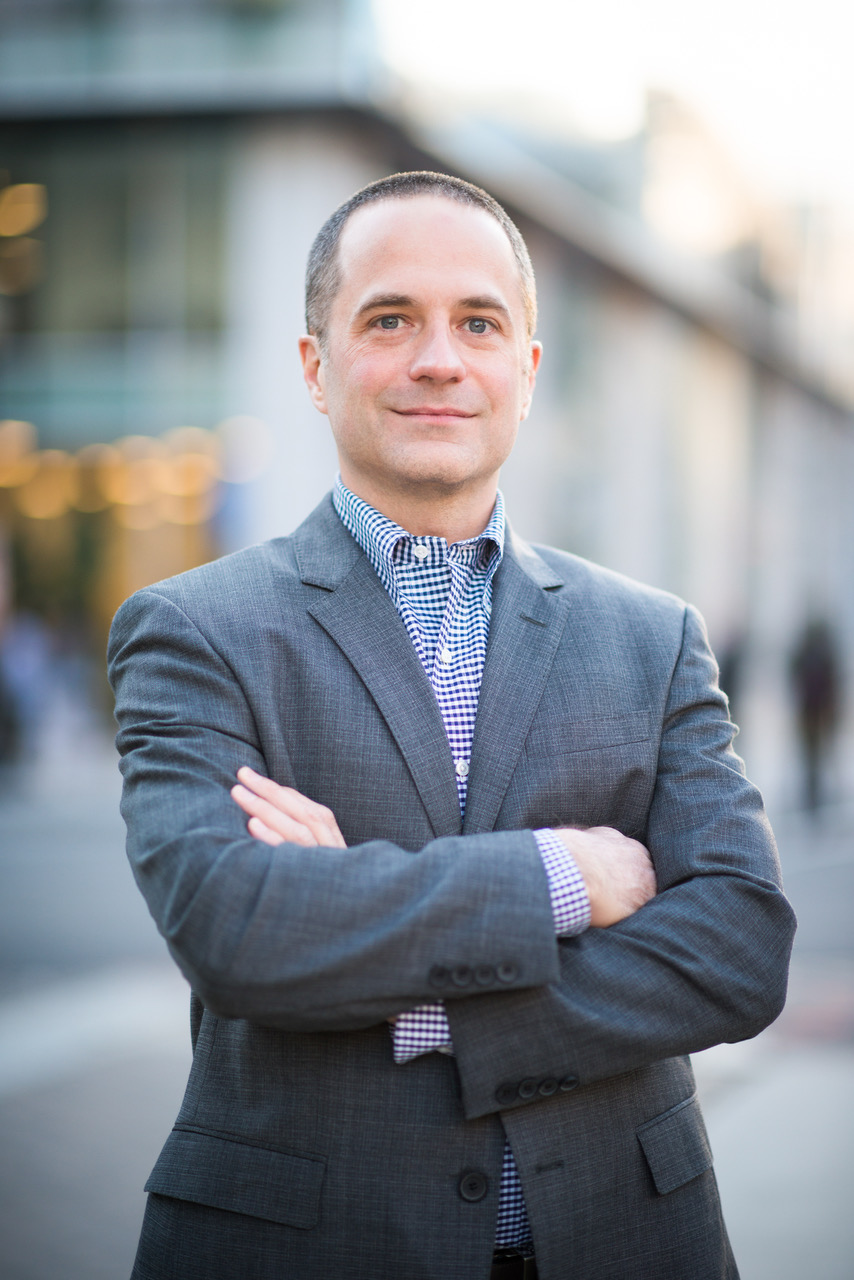
\includegraphics[width=\textwidth,height=0.85\textheight,keepaspectratio]{graphics/Headshot}
            \end{column}
        \end{columns}
    \end{frame}

    \begin{frame}[label=lito]
        \frametitle{Why the JVM?}
        \begin{itemize}
            \item{Reuse the JVM code already in your organization.}
            \item<2->{Reuse the vast amount of Open Source JVM code.}
            \item<3->{Language choices!\pause
               \begin{itemize}
                  \item<4->{Java}
                  \item<4->{Kotlin}
                  \item<4->{Groovy}
                  \item<4->{Scala}
                  \item<4->{Clojure}
                  \item<5->{Java + Kotlin Joint Compilation}
                  \item<5->{Java + Scala Joint Compilation}
               \end{itemize}
            }\pause

        \end{itemize}
        \note<5->[item]{Joint compilation is not Cross Compilation.}
    \end{frame}

    \begin{frame}[label=lito]
        \frametitle{Why GraalVM?}
        \begin{itemize}
            \item<1->{You can be just as cool as the Go and Rust folks (native binaries).}
            \item<2->{Faster startup (a must for CLI tools).}
        \end{itemize}
        \note<1->[item]{No Cross Compilation.}
    \end{frame}

    \begin{frame}[label=lito]
        \frametitle{Gotchas}
        \begin{itemize}
           \item{GraalVM does static analysis, and gets rid of things it thinks aren't used.}
           \item{Static analysis doesn't find code called \emph{only} via reflection. (Use hints\footnotemark[1])}
        \end{itemize}
        %\footnotetext[1]{\resizebox{\hsize}{!}{\url{https://www.graalvm.org/latest/reference-manual/native-image/metadata/\#reflection}}}
        \footnotetext[1]{\resizebox{\dimexpr\hsize-0.75em\relax}{!}{\url{https://www.graalvm.org/latest/reference-manual/native-image/metadata/\#reflection}}}

            %\item{org.graalvm.nativeimage.MissingReflectionRegistrationError: \\
            %   The program tried to reflectively invoke method \\
            %   public void net.edmacdonald.jvmcli.command.ShowHistory.setDirectory(java.lang.String) \\
            %   without it being registered for runtime reflection. \\
            %   Add public void net.edmacdonald.jvmcli.command.ShowHistory.setDirectory(java.lang.String) to the reflection metadata to solve this problem. \\
            %   See https://www.graalvm.org/latest/reference-manual/native-image/metadata/#reflection for help.}
    \end{frame}

    \begin{frame}[label=lito]
       \frametitle{CLI Rules (My Soapbox)}
       \begin{itemize}
          \item<1->{Newline separated records}
          \item<2->{ONLY records on STDOUT. No field headings. Nothing else.}
          \item<3->{Whitespace separated fields}
          \item<4->{No intra-field whitespace except in last column}
       \end{itemize}
       \visible<5->{
         OR...\\
         Just output Json
      }
       \note<1->[item]{table stakes}
       \note<2->[item]{`docker ps`}
       \note<2->[item]{No one here who's ever used Java believes it can achieve this.}
       \note<3->[item]{can be read by a human, AND parsed by perl, awk, etc}
       \note<4->[item]{allows you to grab first n-1 columns easily; dump everything else into nth column}
       \note<5->[item]{See? I can adapt. All praise `jq`}
    \end{frame}

%    \begin{frame}
%        \frametitle{How do you use it?}
%        \begin{itemize}
%            \item{Package your Application components as Containers.}\pause
%            \item{Run the Containers in Kubernetes Pods.}\pause
%            \item{Let Kubernetes manage the Pods for you!}
%        \end{itemize}
%    \end{frame}
%
%    \begin{frame}
%        \frametitle{Why go through the hassle? (It can be a hassle)}
%        Kubernetes can manage resources for you by:\pause
%        \begin{itemize}
%            \item{Doing what you say: Ask for 100 pods, it gives you 100 pods -- and ensures you always have 100.}\pause
%            \item{Horizontal Autoscaling: Too much traffic? It scales up.}\pause
%        \end{itemize}
%        Once up and running, Kubernetes can ease some operational burdens:\pause
%        \begin{itemize}
%            \item{Can assign resource quotas at a namespace level.}\pause
%            \item{Can grant access to individuals/groups at a namespace level.}\pause
%            \item{Can manage ingress.}\pause
%            \item{I don't know... find an Ops person and ask them ;-)}\pause
%        \end{itemize}
%        I just know that the Ops team has put all of their guard rails in place.
%        I'm free to create services and roll them out.
%    \end{frame}
%
%    \begin{frame}
%        \frametitle{When can you benefit from horizontal scaling?}
%        \begin{itemize}
%            \uncover<1->{\item{Your app consists only of stateless components.}}
%            \begin{itemize}
%                \uncover<2->{\item{For example: An app that converts uploaded Word documents to PDF documents.}}
%            \end{itemize}
%            \uncover<3->{\item{Your app has stateless and stateful components, but the stateful components are not the bottleneck.}}
%            \begin{itemize}
%                \uncover<4->{\item{Consider SETI@home\footnotemark -- They farmed out intensive computations to a network of PCs, each of which presumably sent back a result that was inserted into their RDBMS.}}
%            \end{itemize}
%            \uncover<5->{\item{You can find a way to scale your stateful components enough that they are no longer the bottleneck.}}
%            \begin{itemize}
%                \uncover<6->{\item{For example: An RDBMS in a read heavy Application can scale read-only replicas horizontally and distribute reads (SELECTs) among them.}}
%                \uncover<7->{\item{Or in a write heavy Application, perhaps the primary entity can be sharded and distributed among multiple RDBMS instances.}}
%            \end{itemize}
%        \end{itemize}
%        \footnotetext[1]<4->{\href{https://en.wikipedia.org/wiki/SETI@home}{https://en.wikipedia.org/wiki/SETI@home}}
%    \end{frame}
%
%    \begin{frame}
%        \begin{center}
%            \Huge High Level Deployment Walkthrough
%        \end{center}
%    \end{frame}
%
%    \begin{frame}<handout:0>
%        \only<1>{\frametitle{Deploying An App: Build Your App}}
%        \only<2>{\frametitle{Deploying An App: Package Your App as a Container}}
%        \only<3>{\frametitle{Deploying An App: Push The Container to a Repository}}
%        \only<4>{\frametitle{Deploying An App: Deploy Pods to a Kubernetes cluster}}
%        \only<5>{\frametitle{Deploying An App: Pods Pull Your Container}}
%
%        \only<1>{\includegraphics[width=\textwidth,height=0.85\textheight,keepaspectratio]{graphics/deploy-00-app.eps}}
%        \only<2>{\includegraphics[width=\textwidth,height=0.85\textheight,keepaspectratio]{graphics/deploy-01-appContainerized.eps}}
%        \only<3>{\includegraphics[width=\textwidth,height=0.85\textheight,keepaspectratio]{graphics/deploy-02-containerToRepo.eps}}
%        \only<4>{\includegraphics[width=\textwidth,height=0.85\textheight,keepaspectratio]{graphics/deploy-03-emptyPods.eps}}
%        \only<5>{\includegraphics[width=\textwidth,height=0.85\textheight,keepaspectratio]{graphics/deploy-04-podsWithContainers.eps}}
%    \end{frame}
%
%    \begin{frame}<beamer:0>
%        \frametitle{Deploying An App}
%        \includegraphics[width=\textwidth,height=0.85\textheight,keepaspectratio]{graphics/deploy-04-podsWithContainers.eps}
%    \end{frame}
%
%    \begin{frame}
%        \begin{center}
%            \Huge Simple, right? Now let's get into the weeds.
%        \end{center}
%    \end{frame}
%
%    \begin{frame}
%        \frametitle{Tools}
%        \begin{itemize}
%            \uncover<1->{\item docker\footnotemark[1]}
%            \begin{itemize}
%                \uncover<2->{\item How we package our Applications and put them in a place where k8s can find them.}
%            \end{itemize}
%            \uncover<3->{\item minikube\footnotemark[2]}
%            \begin{itemize}
%                \uncover<4->{\item Our very own k8s cluster on our laptop (development use only!).}
%            \end{itemize}
%            \uncover<5->{\item helm\footnotemark[3]}
%            \begin{itemize}
%                \uncover<6->{\item How we package and rollout k8s manifests.}
%            \end{itemize}
%            \uncover<7->{\item kubectl\footnotemark[4]}
%            \begin{itemize}
%                \uncover<8->{\item How we Create, Read, Update, and Delete k8s resources (when helm would be overkill).}
%                \uncover<9->{\item Very thin wrapper around k8s API.}
%            \end{itemize}
%        \end{itemize}
%        \footnotetext[1]<1->{\href{https://www.docker.com/get-started}{https://www.docker.com/get-started}}
%        \footnotetext[2]<3->{\href{https://kubernetes.io/docs/tasks/tools/install-minikube}{https://kubernetes.io/docs/tasks/tools/install-minikube}}
%        \footnotetext[3]<5->{\href{https://helm.sh}{https://helm.sh}}
%        \footnotetext[4]<7->{\href{https://kubernetes.io/docs/tasks/tools/install-kubectl}{https://kubernetes.io/docs/tasks/tools/install-kubectl}}
%    \end{frame}
%
%    \begin{frame}
%        \frametitle{Kubernetes Nodes}
%        \begin{itemize}
%            \uncover<1->{\item The (virtual) machines that make up the Kubernetes cluster.}
%            \uncover<2->{\item Kubernetes schedules Pods to run on these Nodes.}
%            \uncover<3->{\item Managed Kubernetes services\footnotemark[1] can change the number of Nodes to increase/decrease compute resources.}
%        \end{itemize}
%        \footnotetext[1]<3->{\href{https://aws.amazon.com/eks/}{EKS}, \href{https://azure.microsoft.com/en-us/products/kubernetes-service}{AKS}, \href{https://cloud.google.com/kubernetes-engine}{GKE}}
%    \end{frame}
%
%% https://www.patrickbaylis.com/posts/2018-10-11-beamer-resizing/
%    \begin{frame}
%        \frametitle{Kubernetes Nodes}
%        \includegraphics[width=\textwidth,height=0.85\textheight,keepaspectratio]{graphics/00-nodes.eps}
%    \end{frame}
%
%    \begin{frame}
%        \frametitle{Manifest Types - K8s Building Blocks}
%        \includegraphics[width=\textwidth,height=0.85\textheight,keepaspectratio]{graphics/manifest-types.eps}
%    \end{frame}
%
%    \begin{frame}
%        \frametitle{Pods}
%        Pods (not Containers!) are the fundamental building blocks of a Kubernetes Application\pause
%        \begin{itemize}
%            \item A Pod is a group of one or more Containers that work closely together on a specific task.\pause
%            \item Pods manage Volumes for their Containers.\pause
%            \item Pods specify health check endpoints for their Containers.
%        \end{itemize}
%    \end{frame}
%
%    \begin{frame}
%        \frametitle{ReplicaSets (Stateless)}
%        \begin{itemize}
%            \item ReplicaSets manage a set of Pods.\pause
%            \item Pods come and go.\pause
%            \begin{itemize}
%                \item Replaced if unresponsive.\pause
%                \item Can be deleted on one Node and added on another (moved).\pause
%                \item \textbf{You cannot prevent either of these things from happening.}\pause
%            \end{itemize}
%            \item With ReplicaSets\pause
%            \begin{itemize}
%                \item Volumes don't follow Pods.\pause
%                \item Hostnames don't follow Pods.
%            \end{itemize}
%        \end{itemize}
%    \end{frame}
%
%    \begin{frame}
%        \frametitle{Deployments}
%        \begin{itemize}
%            \item ReplicaSets with more features. For example: rollout strategies (canary, rolling update).\pause
%            \item I just used one because helm produces them for skeleton helm projects.
%        \end{itemize}
%    \end{frame}
%
%    \begin{frame}
%        \frametitle{Serivce (Load Balancer)}
%        \begin{itemize}
%            \item Load Balancers have an internal cluster IP address.\pause
%            \item They can also have an external IP address.\pause
%            \item They distribute requests sent to either IP address to all Pods targeted by their ``selector".
%        \end{itemize}
%    \end{frame}
%
%    \begin{frame}
%        \frametitle{The Sample App}
%        I wrote an Application that does nothing other than suggest a random Subreddit.\pause
%        \begin{itemize}
%            \item Stateless.\pause
%            \item Selects at random from a list of 280 Subreddits.\pause
%            \item The list never changes.\pause
%            \item It doesn't need to store anything anywhere.
%        \end{itemize}
%    \end{frame}
%
%    \begin{frame}
%        \frametitle{Load Balancers}
%        \includegraphics[width=\textwidth,height=0.85\textheight,keepaspectratio]{graphics/08-loadBalancer.eps}
%    \end{frame}
%
    \begin{frame}[label=all]
        \frametitle{Demo}
        Tech Stack
        \begin{itemize}
           \item{GraalVM}\footnotemark[1] 
           \item{Java}\footnotemark[2] 
           \item{Scala}\footnotemark[3] 
           \item{picocli}\footnotemark[4] 
           \item{Spring}\footnotemark[5] 
           \item{H2}\footnotemark[6] 
           \item{Liquibase}\footnotemark[7] 
           \item{AspectJ}\footnotemark[8] 
        \end{itemize}
        \footnotetext[1]{\url{https://www.graalvm.org/}}
        \footnotetext[2]{\url{https://www.java.com/en/}}
        \footnotetext[3]{\url{https://www.scala-lang.org/}}
        \footnotetext[4]{\url{https://picocli.info/}}
        \footnotetext[5]{\url{https://spring.io/}}
        \footnotetext[6]{\url{https://www.h2database.com/}}
        \footnotetext[7]{\url{https://docs.liquibase.com/community}}
        \footnotetext[8]{\url{https://eclipse.dev/aspectj/}}
        \note{
            Note that every time we startup...
            \begin{itemize}
               \item{Spring is initialized}
               \item{Datbase migration necessity is evaluated}
               \item{Database connection created}
            \end{itemize}
            Notes:
            \begin{itemize}
               \item{sdk env install}
               \item{
                     scripts/run
                     \begin{itemize}
                        \item{fast}
                        \item{useful output; sent to STDERR}
                     \end{itemize}
                  }
               \item{
                     scripts/run -h
                     \begin{itemize}
                        \item{useful output; sent to STDOUT}
                     \end{itemize}
                  }
               \item{
                     scripts/run -v
                     \begin{itemize}
                        \item{It's still Java; It's still Spring}
                     \end{itemize}
                  }
               \item{scripts/run filesys ls .}
               \item{scripts/run filesys find .}
               \item{scripts/run foobar fizzbuzz baz}
               \item{scripts/run history show}
            \end{itemize}
        }
    \end{frame}
%
%    \begin{frame}
%        \frametitle{Prep Work}
%        \begin{itemize}
%            \item Started our Kubernetes environment (minikube).\pause
%            \item Configured our docker cli to talk to minikube's docker host.\pause
%            \item Built our sample Application, packaged it as a docker Container, and pushed the image.\pause
%            \item Ran helm to deploy our Kubernetes components.\pause
%            \item Proxied local ports to connect to our load balancing services.
%        \end{itemize}
%    \end{frame}
%
%    \begin{frame}
%        \frametitle{Demo Architecture}
%        \includegraphics[width=\textwidth,height=0.85\textheight,keepaspectratio]{graphics/simplifiedModel-00.eps}
%    \end{frame}
%
%    \begin{frame}
%        \frametitle{Exercises}
%        \begin{itemize}
%            \item{Kill a Pod. Watch it restart.}
%            \item{Scale up to 10 Pods. We'll see a manifest!}
%            \item{Scale down to 1 Pod.}
%            \item{Look closer at a Deployment manifest.}
%            \begin{itemize}
%                \item{Note the ReplicaSet spec.}
%                \item{Note the Pod spec.}
%            \end{itemize}
%        \end{itemize}
%    \end{frame}
%
%    \begin{frame}
%        \begin{center}
%            \Huge Questions?
%        \end{center}
%    \end{frame}
%
%    \begin{frame}
%        \frametitle{Other Resources}
%        Peripheral tools I used -- some of which warrant their own presentation
%        \begin{itemize}
%            \item \LaTeX: \href{https://www.latex-project.org}{https://www.latex-project.org}
%            \item Beamer: \href{https://ctan.org/pkg/beamer}{https://ctan.org/pkg/beamer}
%            \item Kotlin: \href{https://kotlinlang.org}{https://kotlinlang.org}
%            \item Spring Boot: \href{https://spring.io/projects/spring-boot}{https://spring.io/projects/spring-boot}
%            \item Gradle: \href{https://gradle.org}{https://gradle.org}
%            \item Dia: \href{http://dia-installer.de}{http://dia-installer.de}
%            \item k9s: \href{https://k9scli.io/}{https://k9scli.io/}
%        \end{itemize}
%        \smallskip
%        Where I got my Subreddit data
%        \begin{itemize}
%            \item Bulk Reddit data: \href{http://files.pushshift.io/reddit/subreddits}{http://files.pushshift.io/reddit/subreddits}
%        \end{itemize}
%        Finally, \textbf{\textit{this}} demo
%        \begin{itemize}
%            \item \href{https://github.com/emacdona/k8sdemo}{https://github.com/emacdona/k8sdemo}
%        \end{itemize}
%    \end{frame}
%
%    \begin{frame}
%        \frametitle{A Note on Capitalization}
%        I agonized over which words to capitalize.
%        \begin{itemize}
%            \item{I capitalized important concepts in the Kubernetes domain:}
%            \begin{itemize}
%                \item{Any Kubernetes component: Deployment, Pod, ReplicaSet, StatefulSet, ...}
%                \item{Application, Container, Kubernetes, Node, Volume}
%            \end{itemize}
%
%            \item{But some didn't quite make the cut:}
%            \begin{itemize}
%                \item{cluster, component}
%            \end{itemize}
%
%            \item{I could not bring myself to capitalize things that I type at the command prompt:}
%            \begin{itemize}
%                \item{docker, helm, kubectl, minikube}
%            \end{itemize}
%        \end{itemize}
%    \end{frame}
%
%    \begin{frame}
%        \frametitle{``It Worked on My Machine" Demo Remix}
%        \only<1|handout:1>{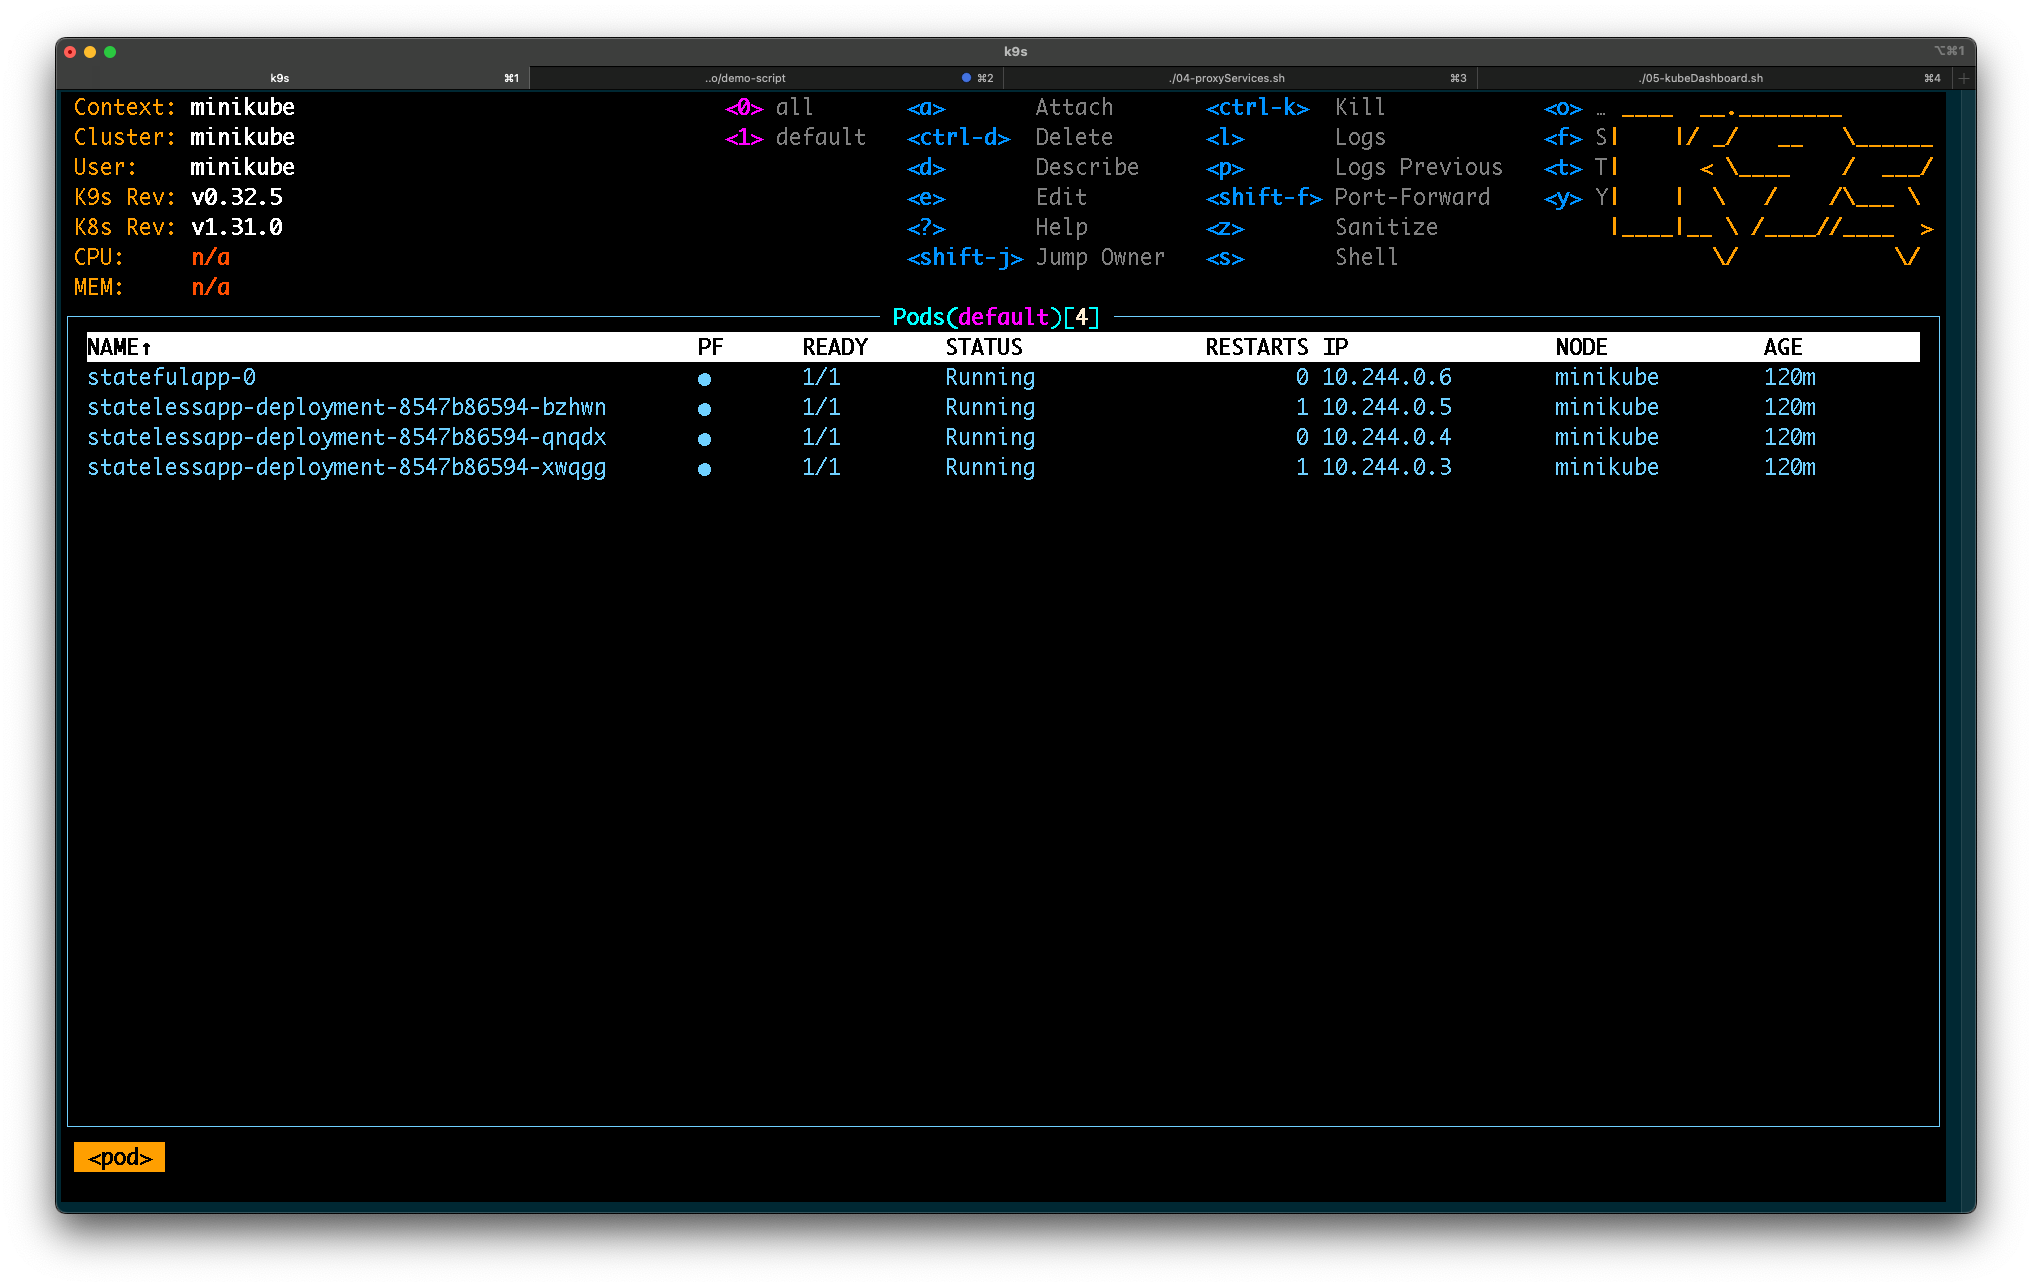
\includegraphics[width=\textwidth,height=0.85\textheight,keepaspectratio]{graphics/screenshots/00-pods}}
%        \only<2|handout:2>{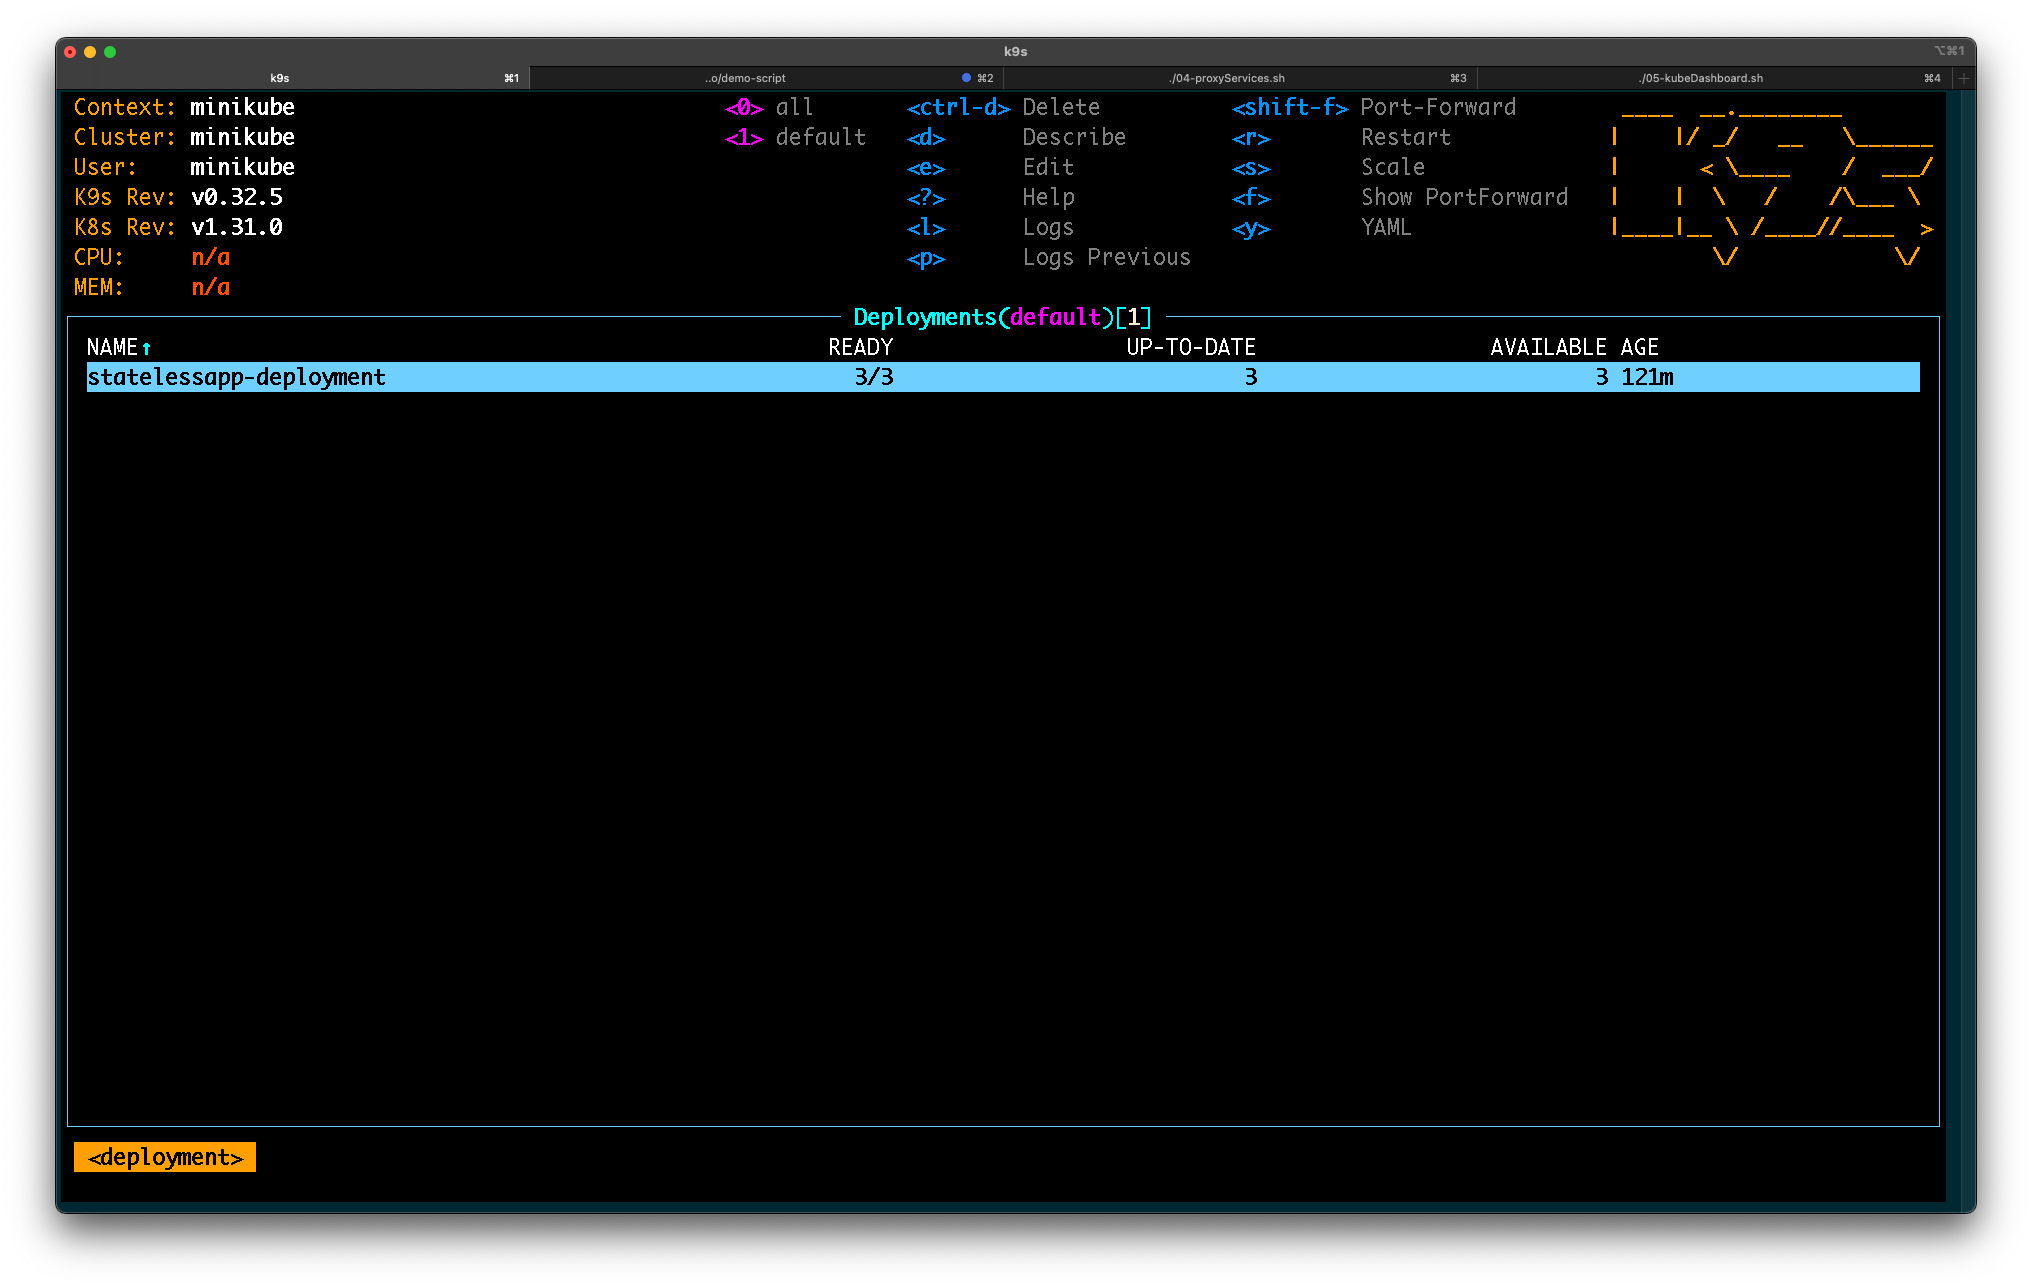
\includegraphics[width=\textwidth,height=0.85\textheight,keepaspectratio]{graphics/screenshots/01-deployment}}
%        \only<3|handout:3>{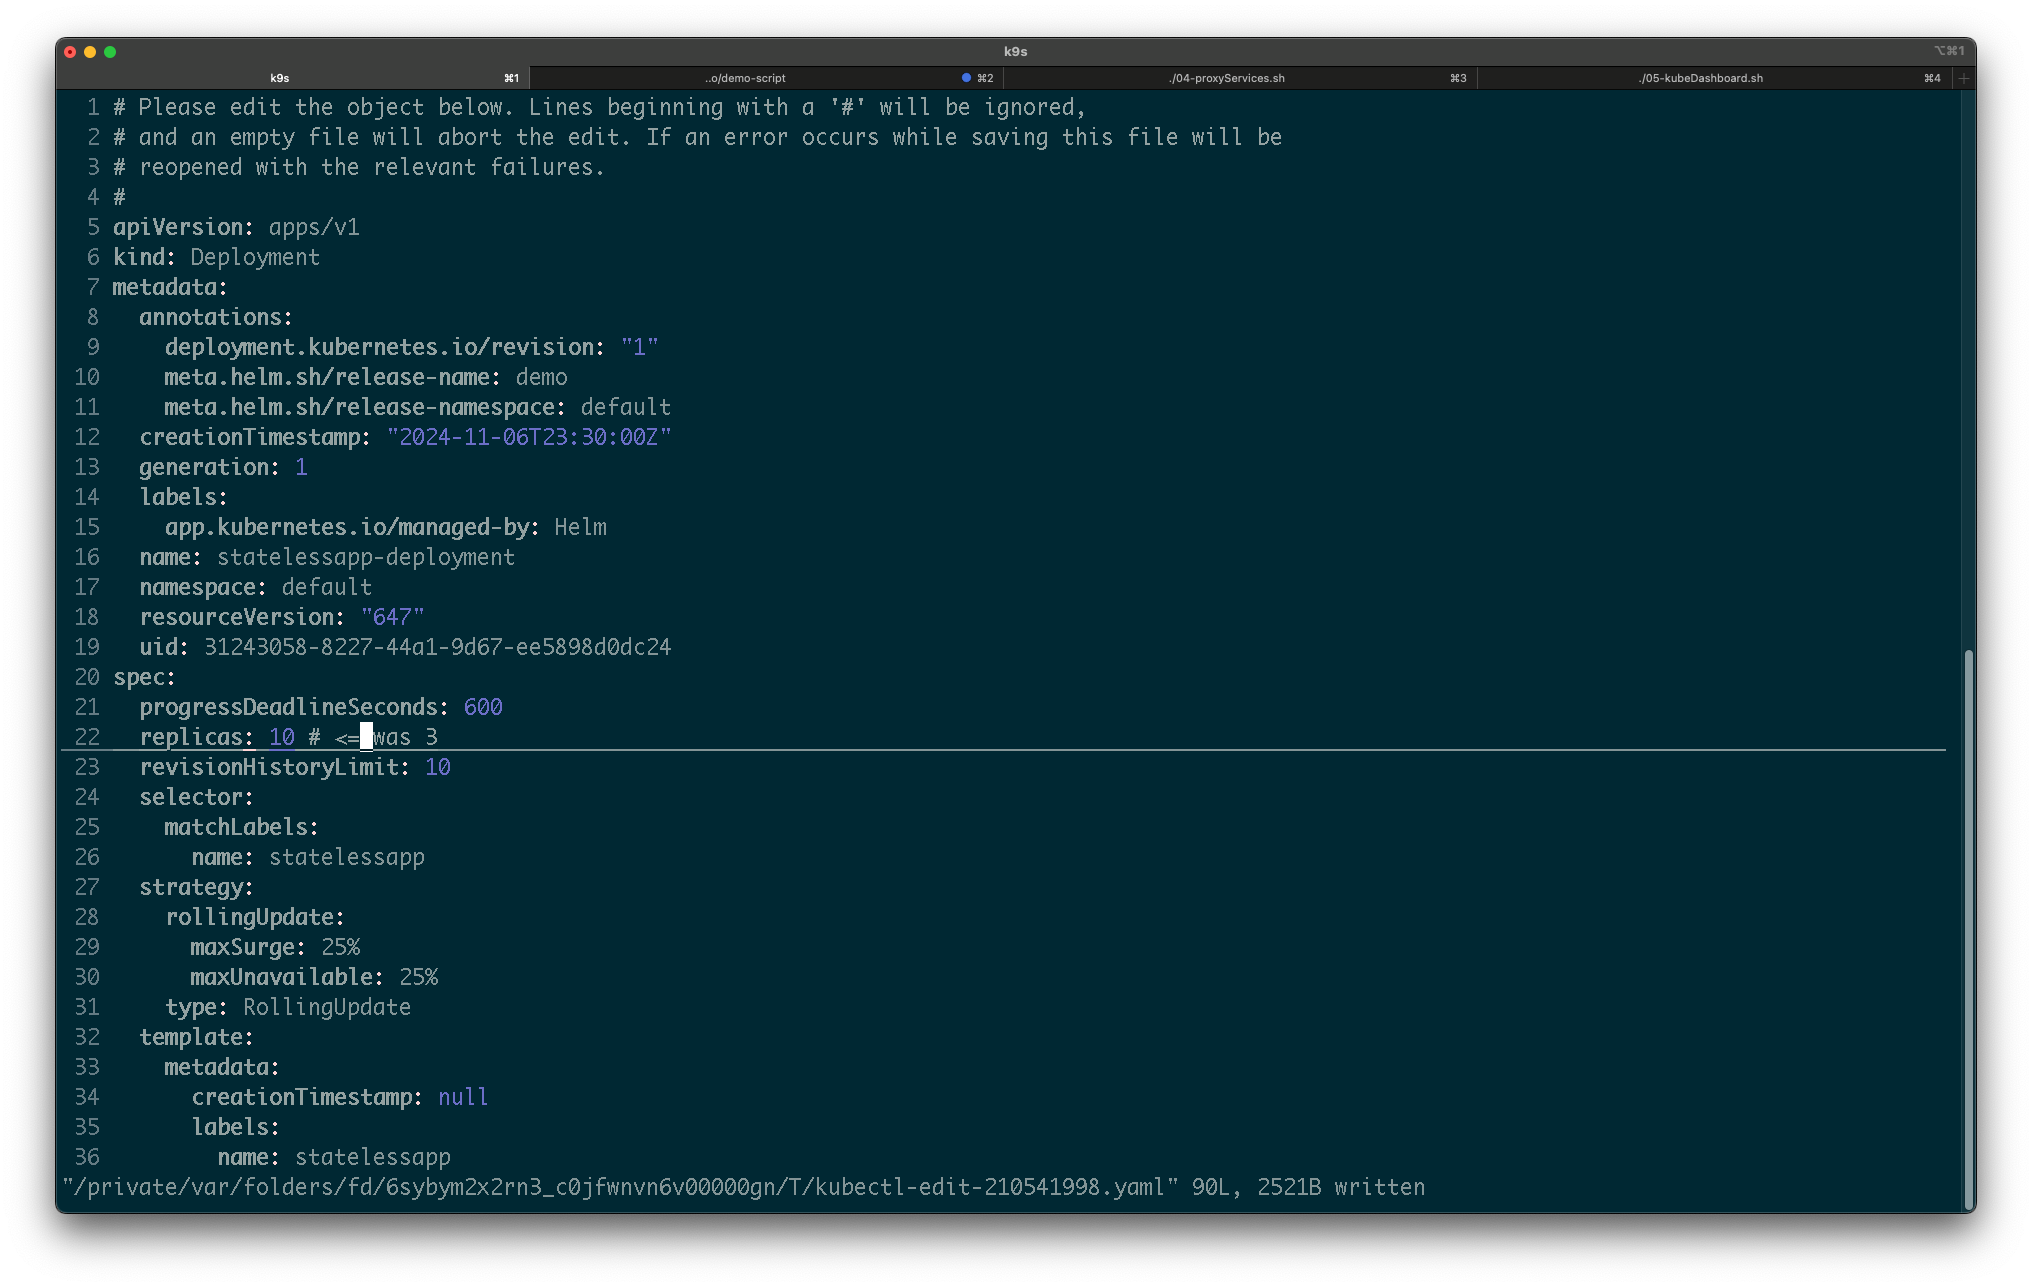
\includegraphics[width=\textwidth,height=0.85\textheight,keepaspectratio]{graphics/screenshots/02-scaleUp}}
%        \only<4|handout:4>{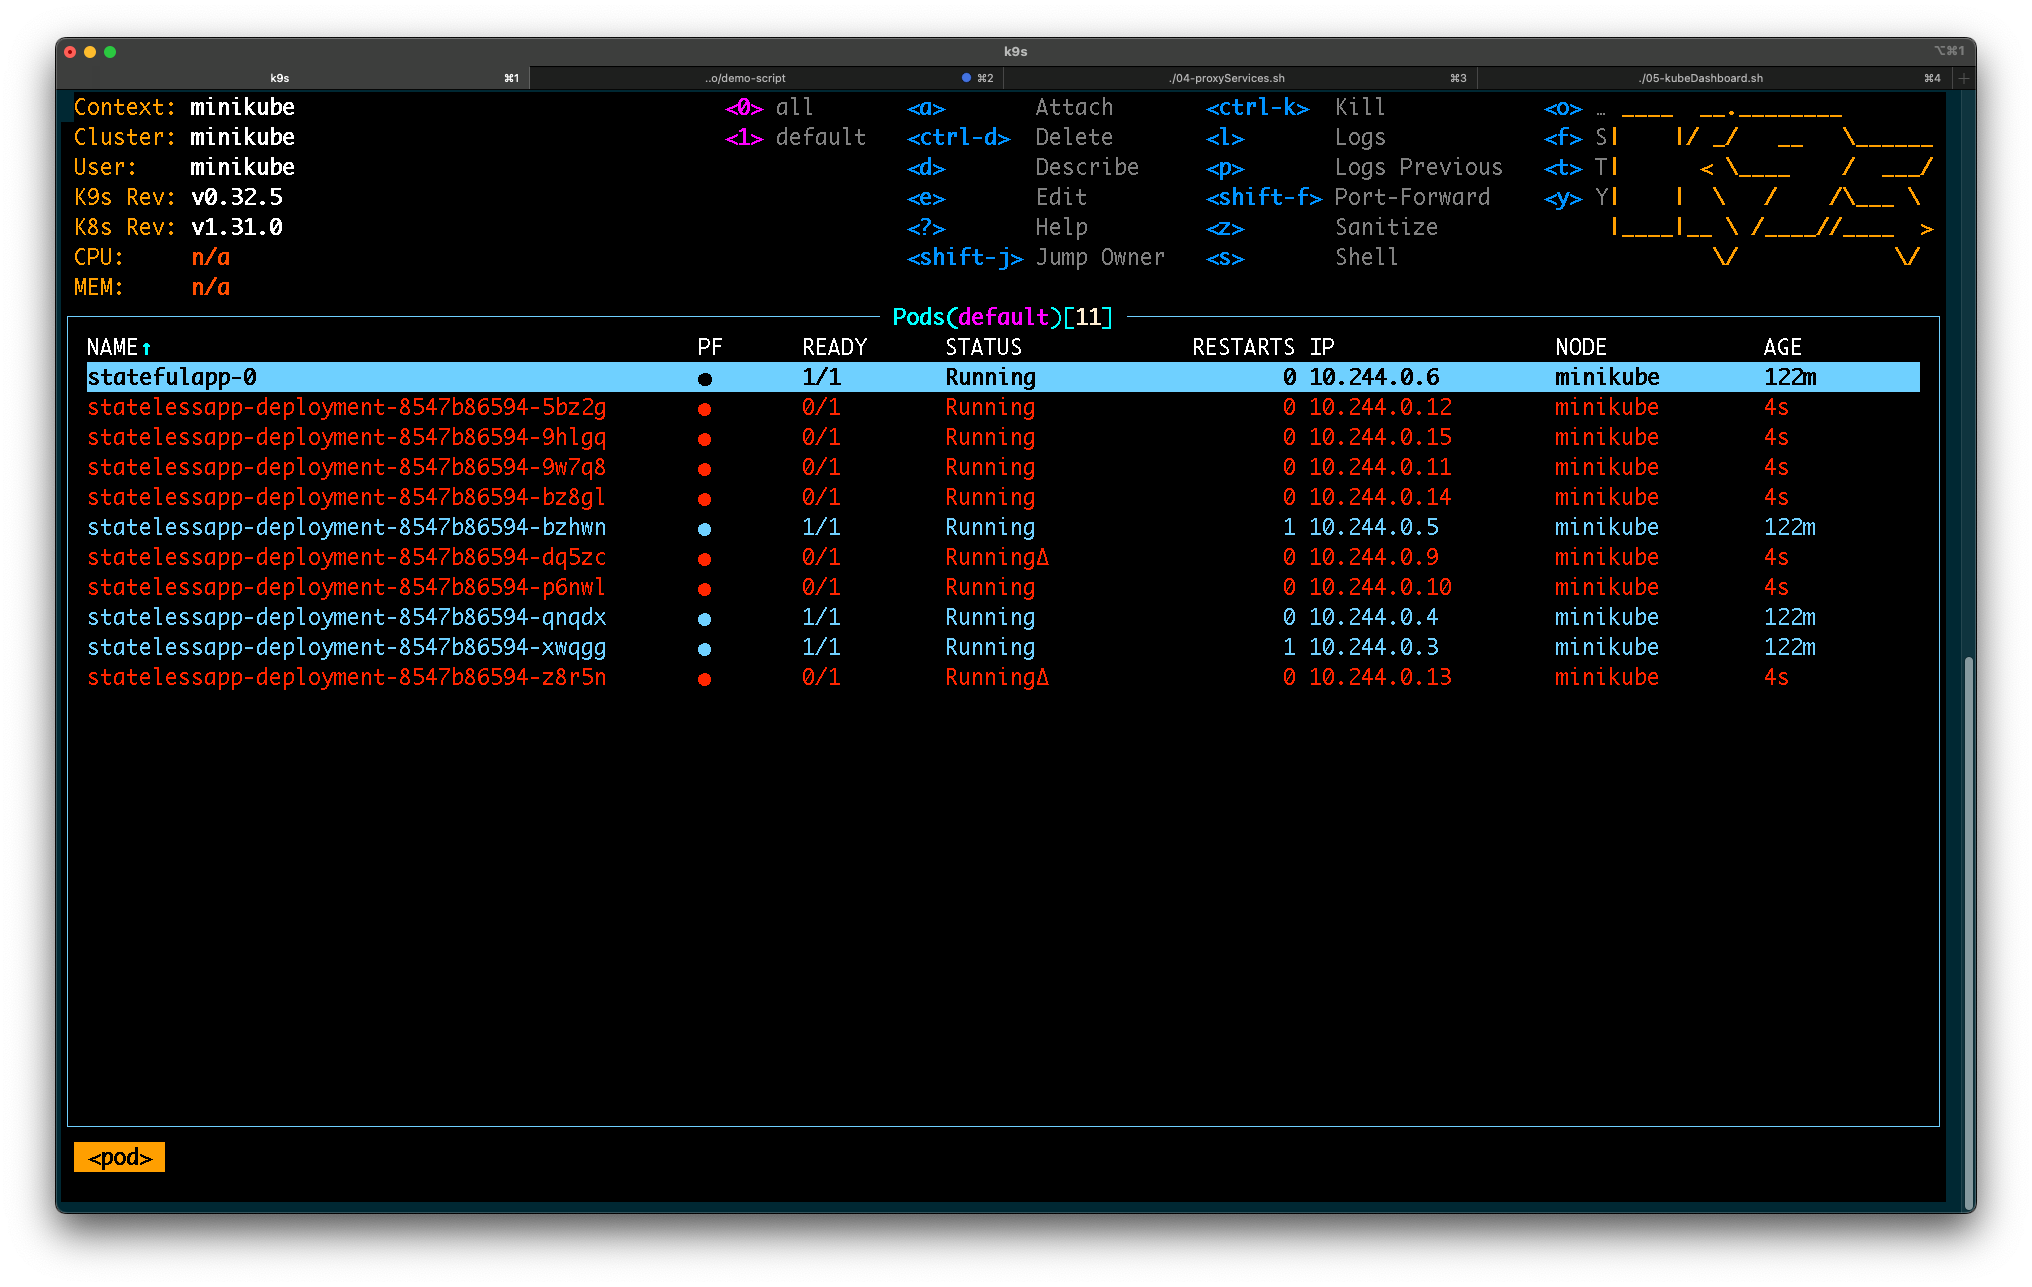
\includegraphics[width=\textwidth,height=0.85\textheight,keepaspectratio]{graphics/screenshots/03-converging}}
%        \only<5|handout:5>{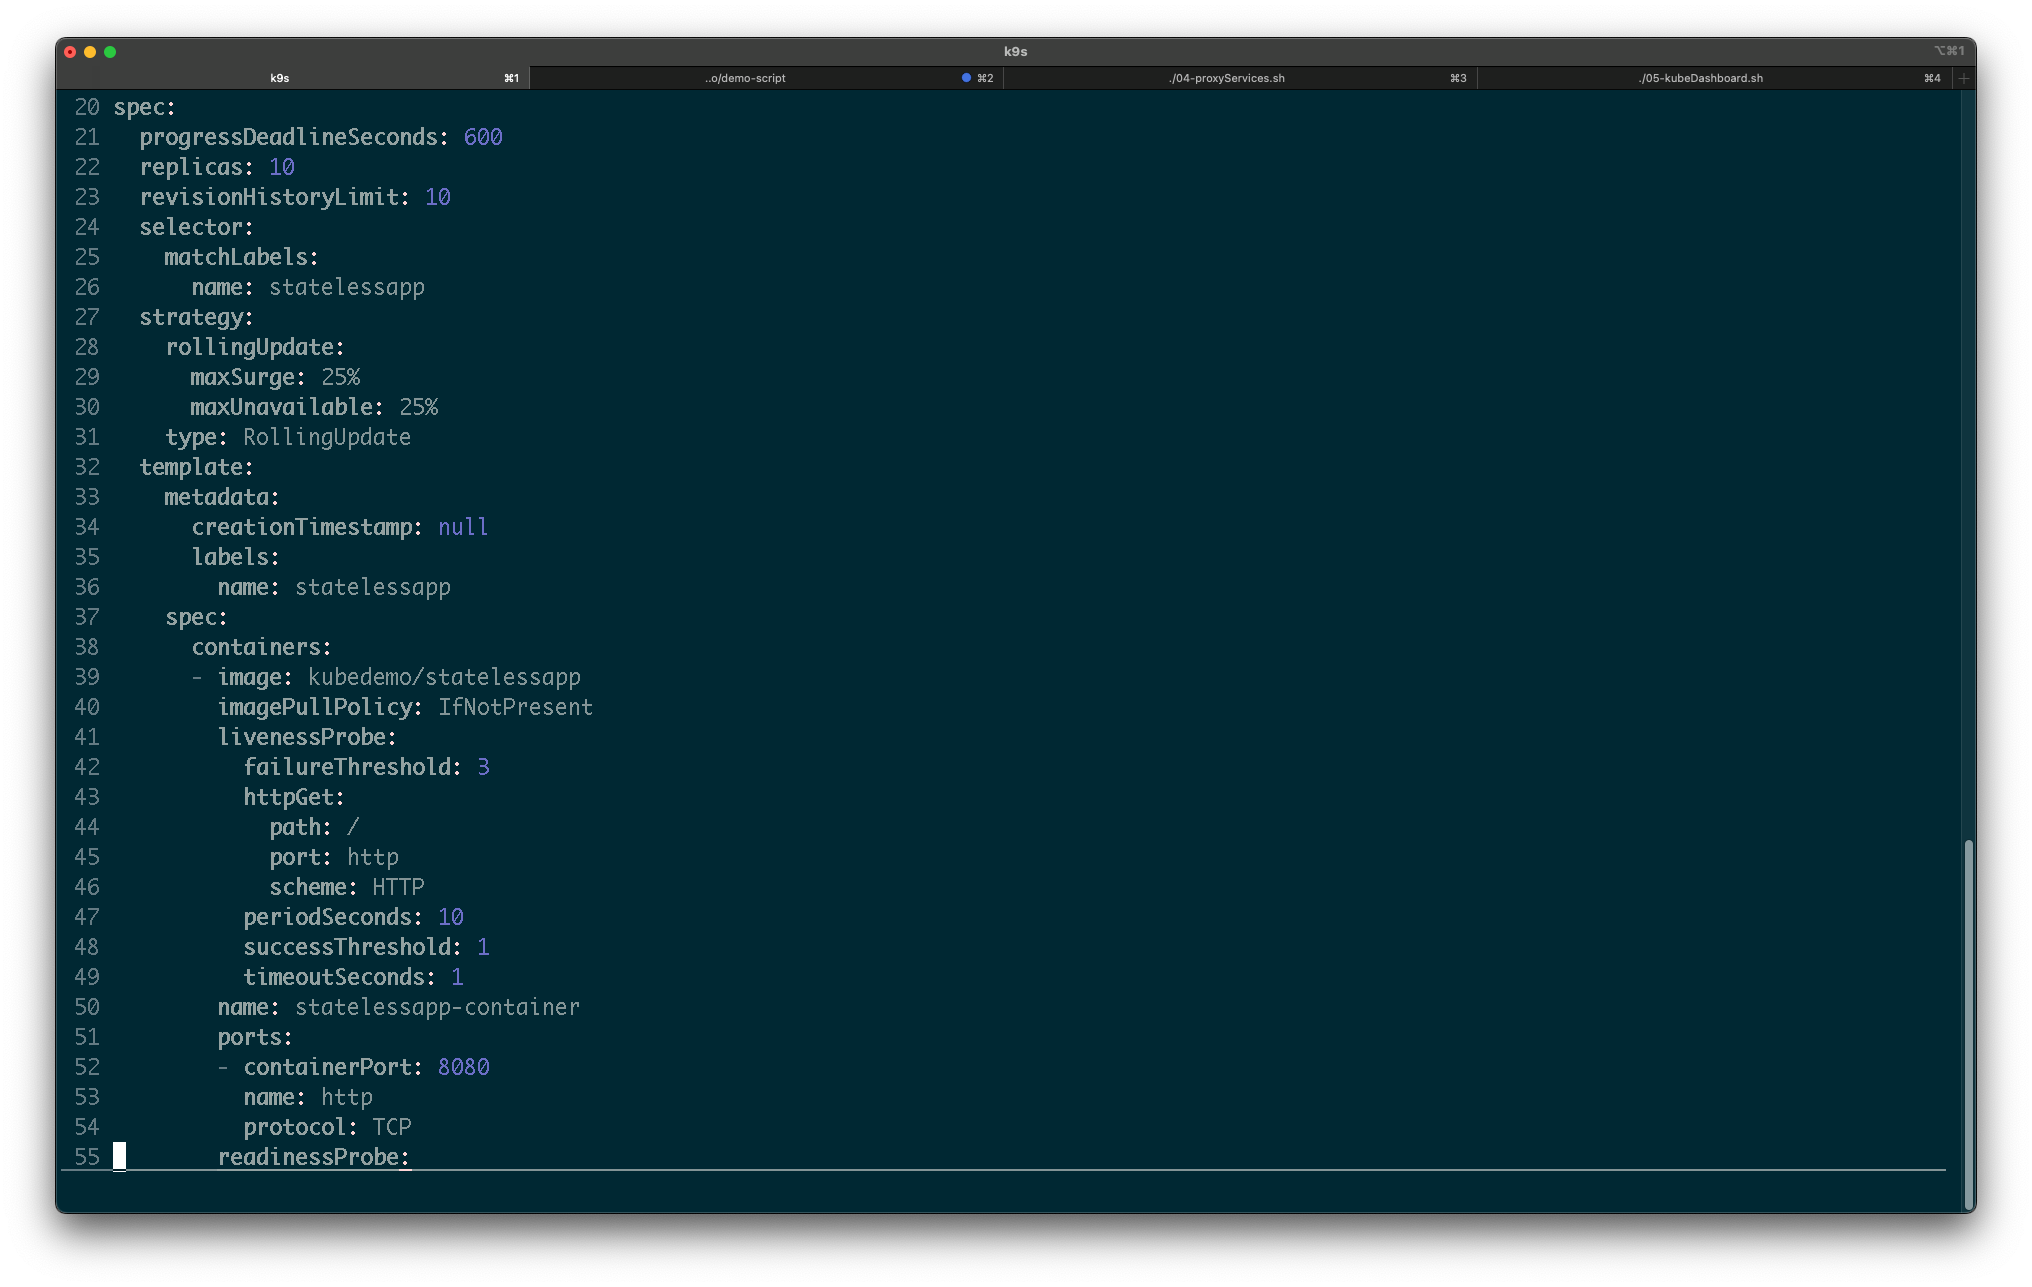
\includegraphics[width=\textwidth,height=0.85\textheight,keepaspectratio]{graphics/screenshots/04-deploymentManifest}}
%    \end{frame}

\end{document}
